% texlive2017, xelatex
% author: Ma Seoyin, 2014 Applied Physics, SCUT
\documentclass{standalone}
\usepackage{bm} % Required for the bold in math display
\usepackage{amsmath} % Required for the math display
\usepackage{tikz, tikzscale}
\usetikzlibrary{shapes.geometric, arrows,calc,positioning,decorations.pathreplacing,bending}

%----------------------------------------------------------------------------------------
%   Flow chart setting
%----------------------------------------------------------------------------------------
%   Define the fundamental shapes of the flow chart
\tikzstyle{StartEnd} = [rectangle, rounded corners, minimum width = 2cm, minimum height=0.6cm,text centered, draw = black, fill = red!40]
\tikzstyle{ioFunction} = [trapezium, trapezium left angle=70, trapezium right angle=110, minimum width=2cm, minimum height=0.6cm, text centered, draw=black, fill = blue!40]
\tikzstyle{process} = [rectangle, minimum width=2cm, minimum height=0.6cm, text centered, draw=black, fill = yellow!50]
\tikzstyle{decision} = [diamond, minimum height=0.8cm,  aspect = 5, text centered, draw=black, fill = green!30]
\tikzstyle{defineRangeSearch} = [rectangle, minimum width=2cm, minimum height=0.6cm, text centered, draw=black, fill = green!30]
%   Define the arrows' shape of the flow chart
\tikzstyle{arrow} = [->,>=stealth]


\begin{document}
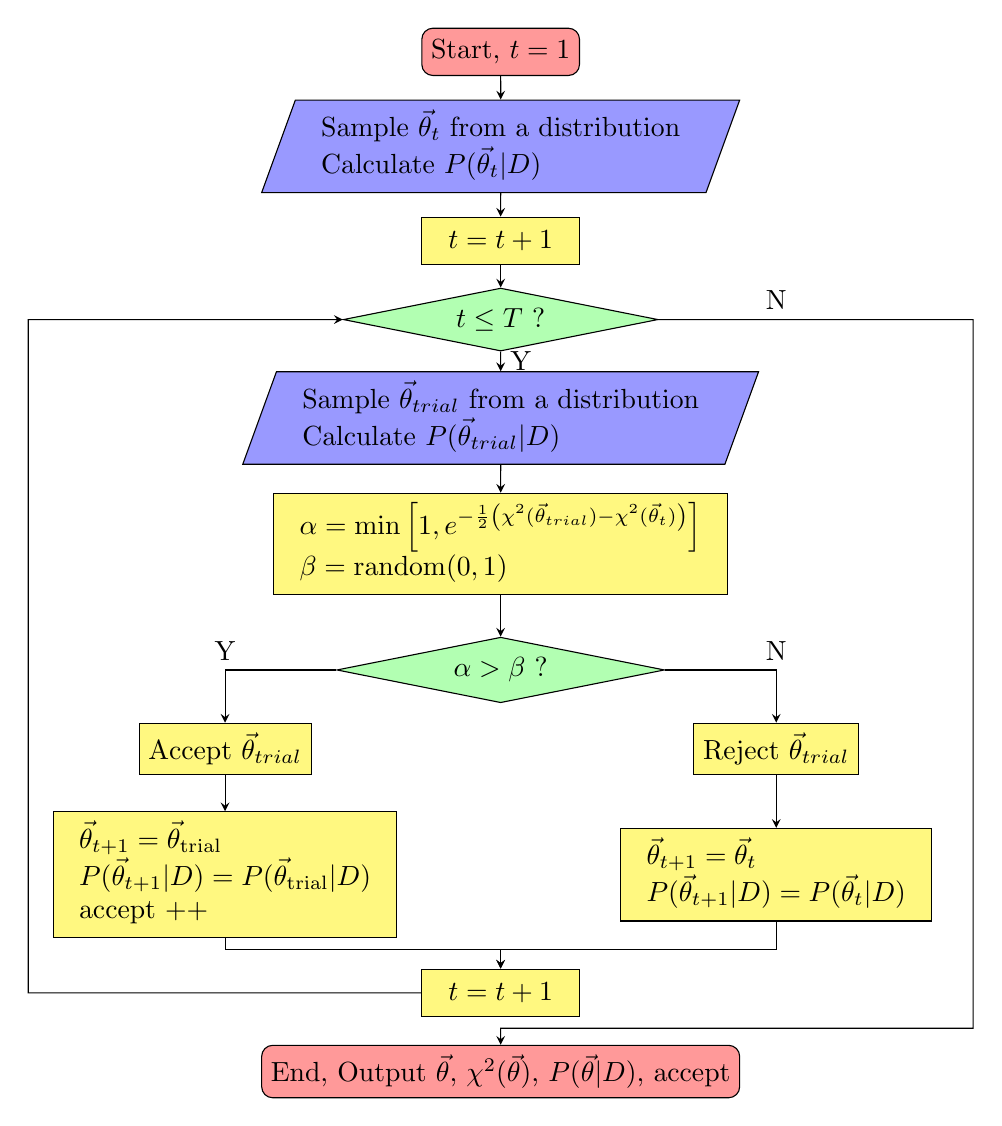
\begin{tikzpicture}[transform shape, node distance=1.0cm]
% Draw shapes
\node (t_1) [StartEnd]
{Start, $t = 1$};
\node (Input) [ioFunction, below of = t_1, node distance=1.2cm]
{\begin{tabular}{l}
Sample $\vec{\theta}_t$ from a distribution\\
Calculate $P(\vec{\theta}_{t}|D)$\\
\end{tabular}};
\node (t_2) [process, below of = Input, node distance=1.2cm]
{$t = t + 1$};
\node (iteration) [decision, below of = t_2]
{$t \leq T$ ?};
\node (trial) [ioFunction, below of = iteration, node distance = 1.25cm]
{\begin{tabular}{l}
Sample $\vec{\theta}_{trial}$ from a distribution\\
Calculate $P(\vec{\theta}_{trial}|D)$\\
\end{tabular}};
\node (alpha_beta) [process, below of = trial, node distance = 1.6cm]
{\begin{tabular}{l}
$\alpha=\min\left[1, e^{-\frac12\left(\chi^2(\vec{\theta}_{trial}) - \chi^2(\vec{\theta}_{t})\right)}\right]$\\
$\beta={\rm random}(0,1)$\\
\end{tabular}};
\node (If_alpha_beta) [decision, below of = alpha_beta, node distance=1.6cm]
{$\alpha > \beta\ ?$};
\node (Accept) [process, below of = If_alpha_beta, xshift=-3.5cm]
{Accept $\vec{\theta}_{trial}$};
\node (AcceptUpdate) [process, below of = Accept, node distance=1.6cm]
{\begin{tabular}{l}
$\vec{\theta}_{t+1}=\vec{\theta}_{\rm trial}$\\
$P(\vec{\theta}_{t+1}|D)=P(\vec{\theta}_{\rm trial}|D)$\\
accept ++\\
\end{tabular}};
\node (Reject) [process, below of = If_alpha_beta, xshift=3.5cm]
{Reject $\vec{\theta}_{trial}$};
\node (RejectUpdate) [process, below of = Reject, node distance=1.6cm]
{\begin{tabular}{l}
$\vec{\theta}_{t+1}=\vec{\theta}_{t}$\\
$P(\vec{\theta}_{t+1}|D)=P(\vec{\theta}_{t}|D)$\\
\end{tabular}};
\node (t_plus_1) [process, below of = If_alpha_beta, node distance = 4.1cm]
{$t = t + 1$};
\node (End) [StartEnd, below of = t_plus_1]
{End, Output $\vec{\theta}$, $\chi^2(\vec{\theta})$, $P(\vec{\theta}|D)$, accept};
% Draw arrows
\draw [arrow] (t_1) -- (Input);
\draw [arrow] (Input) -- (t_2);
\draw [arrow] (t_2) -- (iteration);
\draw [arrow] (iteration) -- node [right] {Y} (trial);
\draw [arrow] (trial) -- (alpha_beta);
\draw [arrow] (alpha_beta) -- (If_alpha_beta);
\draw [arrow] (If_alpha_beta) -| node [above] {Y} (Accept);
\draw [arrow] (If_alpha_beta) -| node [above] {N} (Reject);
\draw [arrow] (Accept) -- (AcceptUpdate);
\draw [arrow] (AcceptUpdate) |- (0,-11.4) -- (t_plus_1);
\draw [arrow] (Reject) -- (RejectUpdate);
\draw [arrow] (RejectUpdate) |- (0,-11.4) -- (t_plus_1);
\draw [arrow] (t_plus_1) -| (-6,-3.4) -- (iteration);
\draw [arrow] (iteration) -- (6,-3.4) node [above, xshift=-2.5cm] {N} |- (0,-12.4) -- (End);
\end{tikzpicture}
\end{document}